\section{Introduction}
\label{sec:intro}


Story understanding task which is an interesting and challenging task for Computational Linguists\cite{mani2012computational}. Since story comprehension is an complex task involving not only the semantic of each sentences or words, but many commonsense knowledge and an understanding of normative social behaviour \cite{charniak1972toward}. Rocstory cloze task in 2016~\cite{mostafazadeh2016corpus} is proposed to evaluate the ability of story comprehension, albeit without the aspect of ending generation, this task gives four sentences plot for read and two alternative endings for choocing. \figref{fig:shanshan1} shows an example story consisting of a short context, and two ending options.

%
\begin{figure}[th]
	\centering
	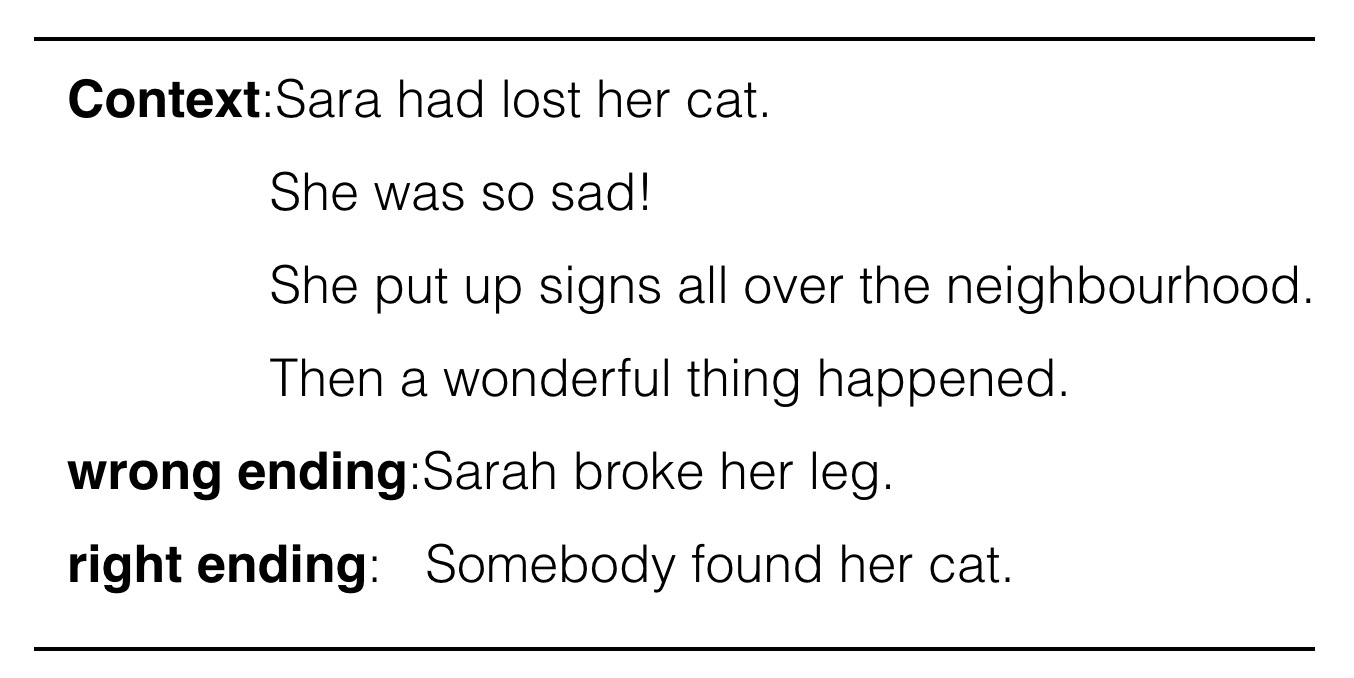
\includegraphics[width=1.0\columnwidth]{figures/shanshan1}
	\caption{An example from the story-cloze task: predict the correct ending to a given short story out of provided options.}
	\label{fig:shanshan1}
\end{figure}
%
In addition, \citeauthor{mostafazadeh2016corpus}\shortcite{mostafazadeh2016corpus} gives 98161 5-sentence stories without negative ending. Consequently, past research mostly training on two different dataset: the 5-sentences training set(denoted TS)~\cite{roemmele2017rnn,wang2017conditional}, more commonly,many research \cite{srinivasan2018simple,chaturvedi2017story,cai2017pay,li2018story} train the supervised model with part of validation set(denoted VS) which has 1871 storys with negative ending. To address the complexity of story reasoning, some supervised training model tried to get different features manually, \citeauthor{chaturvedi2017story}\shortcite{chaturvedi2017story}involves three distinct semantic aspects: (i) the sequence of events described in the story, (ii) its emotional trajectory, and (iii) its plot consistency. \citeauthor{li2018story}\shortcite{li2018story}add five features(i) word embedding, (ii) character feature, (iii) part-of-speech (POS) tagging, (iv) sentiment polarity of a word, and (v) negation to assist feature extraction. Other models \cite{srinivasan2018simple,cai2017pay,roemmele2017rnn} use neural network extract features automatically.
%

We mainly train our model on large training set TS. Because we demonstrate training model on VS is unreasonable. If we only train the model with two alternative ending with no plots, we can also get accuracy 74.3\%. Intuitively, if human choose an ending by only reading two ending sentences, the accuracy should not be so high. Ten volunteers are asked to answer this only ending task with 100 single choice question, the average accuracy is 60\%. Therefore I suppose the endings in validation have similiar distribution with test set. Training on VS transfer this story reasoning task into a combined issue that consists of story reasoning and learning ending distribution task. The improvment on test set can not prove the better performance on story reasoning. Most research may stack in a wrong direction. Therefore, we generate negative data for TS in the similiar method with \citeauthor{roemmele2017rnn}\shortcite{roemmele2017rnn}'s . the score for only training on endings is 59.8\%. 
%

In this paper,our best result obtains 69.2\% accuracy on the test set, outperforming \citeauthor{roemmele2017rnn}\shortcite{roemmele2017rnn}'s best result of 67.2\% on TS. Except that we can also get 79.4\% for training on VS. We use a structural neural network constituted of convolutional neural network(CNN) and recurrent neural network(RNN) to do a binary classifier to distinguish correct story endings from artificially generated incorrect endings. We compare the results for former  best model and our model training on these 2 dataset. Besides, I will compare the model with different structure.
%
Our key contributions are:
%
\begin{itemize}
	\item we proposed a efficient story structural neural network model and get the state of art no matter on TS or VS.
	\item we find the irrational of most research which train on VS.
\end{itemize}
%










